% ----------------------- TODO ---------------------------
% Diese Daten müssen pro Blatt angepasst werden:
\newcommand{\NUMBER}{1}
\newcommand{\EXERCISES}{2}
% Diese Daten müssen einmalig pro Vorlesung angepasst werden:
\newcommand{\COURSE}{Design \& Synthesis of ES}
\newcommand{\TUTOR}{Sebastian Walter}
\newcommand{\STUDENTA}{Alexander Ritter}
\newcommand{\STUDENTB}{Jonas Taigel}
\newcommand{\STUDENTC}{}
\newcommand{\DEADLINE}{11.05.2025}
% ----------------------- TODO ---------------------------

\documentclass[a4paper]{scrartcl}
% https://de.overleaf.com/learn/latex/German#Font_encoding
% To make text better to copy
\usepackage[T1]{fontenc}

\usepackage[utf8]{inputenc}
\usepackage[ngerman]{babel}
\usepackage{amsmath}
\usepackage{amssymb}
\usepackage{fancyhdr}
\usepackage{color}
\usepackage{graphicx}
\usepackage{lastpage}
\usepackage{listings}
\usepackage{tikz}
\usepackage{pdflscape}
\usepackage{subfigure}
\usepackage{float}
\usepackage{polynom}
\usepackage{hyperref}
\usepackage{tabularx}
\usepackage{forloop}
\usepackage{geometry}
\usepackage{listings}
\usepackage{fancybox}
\usepackage{tikz}
\usepackage{enumitem}

%Größe der Ränder setzen
\geometry{a4paper,left=3cm, right=3cm, top=3cm, bottom=3cm}

%Kopf- und Fußzeile
\pagestyle {fancy}
\fancyhead[L]{Tutor: \TUTOR}
\fancyhead[C]{\COURSE}
\fancyhead[R]{\today}

\fancyfoot[L]{}
\fancyfoot[C]{}
\fancyfoot[R]{Seite \thepage /\pageref*{LastPage}}

%Formatierung der Überschrift, hier nichts ändern
\def\header#1#2{
  \begin{center}
    {\Large Übungsblatt #1}\\
    {(Abgabetermin #2)}
  \end{center}
}

%Definition der Punktetabelle, hier nichts ändern
\newcounter{punktelistectr}
\newcounter{punkte}
\newcommand{\punkteliste}[2]{%
  \setcounter{punkte}{#2}%
  \addtocounter{punkte}{-#1}%
  \stepcounter{punkte}%<-- also punkte = m-n+1 = Anzahl Spalten[1]
  \begin{center}%
  \begin{tabularx}{\linewidth}[]{@{}*{\thepunkte}{>{\centering\arraybackslash} X|}@{}>{\centering\arraybackslash}X}
      \forloop{punktelistectr}{#1}{\value{punktelistectr} < #2 } %
      {%
        \thepunktelistectr &
      }
      #2 &  $\Sigma$ \\
      \hline
      \forloop{punktelistectr}{#1}{\value{punktelistectr} < #2 } %
      {%
        &
      } &\\
      \forloop{punktelistectr}{#1}{\value{punktelistectr} < #2 } %
      {%
        &
      } &\\
    \end{tabularx}
  \end{center}
}

\begin{document}

\begin{tabularx}{\linewidth}{m{0.2 \linewidth}X}
  \begin{minipage}{\linewidth}
    \STUDENTA\\
    \STUDENTB\\
    \STUDENTC
  \end{minipage} & \begin{minipage}{\linewidth}
    \punkteliste{1}{\EXERCISES}
  \end{minipage}\\
\end{tabularx}

\header{Nr. \NUMBER}{\DEADLINE}



% ----------------------- TODO ---------------------------
% Hier werden die Aufgaben/Lösungen eingetragen:

\section*{Aufgabe 1}
\begin{enumerate}[label=(\alph*)]

    \item 
    The different layers of abstraction model the functionality of the system at differing complexities.
    This makes it possible for the designer to understand the system at one abstraction level without needing to know the exact details of the abstraction level below. 
    \\\\
    For the transformation between levels, there are synthesis steps which are
        \begin{itemize}
            \item High-Level Synthesis: Synthesizes a register-transfer-level system that performs the given algorithm 
            \item RT Synthesis: Realizes the Register-Transfer system in individual logic components
            \item Logic Synthesis: Translates from the logic level (gates, flipflops, complex components) down to the circuit level (transistors and electrophysics) 
        \end{itemize}
        
    
    \item 
    The main difference is that the behavioral view does not think about the components and architecture and rather about how the systems functions.
    For example we have an Alarm System that activates automatically at night and deactivates during daytime.
    \begin{itemize}
        \item Behavioral View: If the alarm system detects daylight, the alarm is turned off until daylight is no longer detected. Then, the system automatically turns the alarm back on until daylight is detected again.
        \item Structural View: The system consists of a daylight sensor that continuously sends a logical signal, the alarm management system and a bus that transmits the logical signal to the management system.
    \end{itemize}

    \item 
    Intellectual property is the legal concept of protecting an invention, giving all rights to the creator only, thereby allowing the creator to monetize it for a time. For example patents and copyright ensure exclusive production and selling.
    In chip development, the term is used by chip/design creators to refer to components or architecture designs that are licensed to users that want to build or sell a system using those components.\\
    These so called IP cores can be soft (code in a HDL like SystemVerilog for example), or hard (the chip layout is already given) \footnote{https://de.wikipedia.org/wiki/IP-Core}.
    

    \item 
    The main difference lies in the flexibility of the chips. The FPGA can still be changed in how it works after fabrication while the ASIC chip has a fixed design in which its fabricated. 
    The ASIC requires maximum effort during the design, but can be tailored specifically to the use-case because standard cells can be freely combined, thus chip size and number of cells are variable.
    In contrast, FPGAs are manufactured always the same, i.e. the number of gates and wires is fixed, but they can be reprogrammed.
    Because the FPGAS are not optimized or designed for a specific use case the cost of production is significantly higher than in ASICs, which are optimized and because of this can be produced with much lower costs.
    % ...
    % About a factor of 10 smaller clock frequency and lower gate density than a full custom ASIC implementation
    
\end{enumerate}

\section*{Aufgabe 2}
\begin{enumerate}[label=(\alph*)]

\item 
First of all, the half adder should XOR the inputs to calculate the sum bit. Additionally, there is a small syntax error in the form of a comma after the last logic output in the input/output list.
\begin{figure}[h]
    \centering
    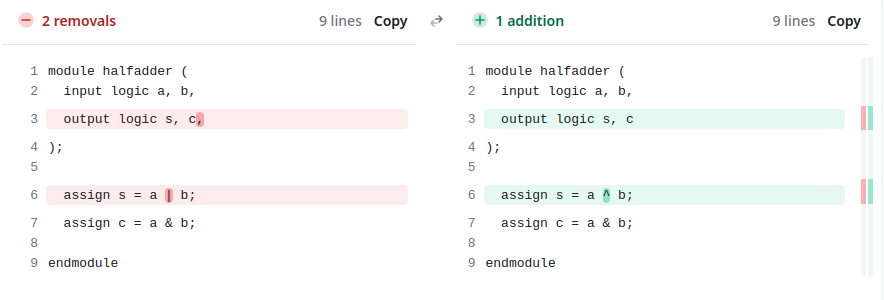
\includegraphics[width=1.0\linewidth]{halfadder-diff.png}
    \caption{Difference between erroneous halfadder (left) and our fixed code (right).}
    \label{fig:halfadder-diff}
\end{figure}

\item 
The halfadder behaves as shown and expected, verified in the \verb|halfadder.vcd| file.
\begin{table}[h]
\centering
\begin{tabular}{ll|ll}
\hline
\textbf{a} & \textbf{b} & \textbf{s} & \textbf{c} \\ \hline
0 & 0 & 0 & 0 \\
0 & 1 & 1 & 0 \\
1 & 0 & 1 & 0 \\
1 & 1 & 0 & 1 \\ \hline
\end{tabular}
\end{table}

\item 
The fulladder is implemented in \verb|fulladder.sv|.
% Fulladder structural using one-bit-halfadder
\begin{figure}[H]
    \centering
    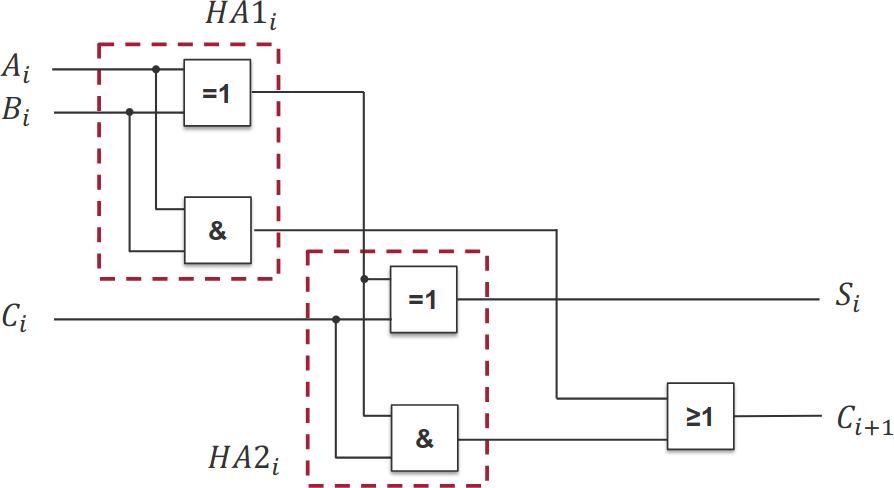
\includegraphics[width=0.6\linewidth]{fulladder.png}
    \caption{Full-adder circuit, Source: TI1 06 page 38, Prof. Dr. Oliver Bringmann}
    \label{fig:fulladder-circuit}
\end{figure}

\item 
% Fulladder vcd
\verb|fulladder.vcd|

\item 
% e) Create the behavioural description of a one-bit full adder in SystemVerilog.
The behavioral description of the full adder simply requires implementing the logic using boolean operations.

\item 
% f) Simulate the behavioural description of the one-bit full adder completely and manually via the command line of Xcelium as in task 2(b). Submit your simulation results as a VCD (Value Change Dump) file.
\verb|fulladder_behavioral.vcd|

\item 
% g) Are the simulation results of the structural description and the behavioural description identical? Explain what differences/similarities you see?
The inputs and outputs are identical, as we realized the same function. The difference we notice is that the VCD of the behavioral full adder contains the waveform simulation for the individual half-adders and their inputs/outputs (called $\text{first},\ \text{second}$ in our file), as well as for the wires (called $\text{carry}_1, \text{carry}_2, \text{sum}_2$) we specified connecting the half-adders. The behavioral full adder just simulates $a, b, c_{in}, s, c_{out}$ directly.

\item 
% h) Create a file and.sv and a SystemVerilog module that describes the behaviour of a logical AND function. Create another file mult.sv and develop a structural description of a 3-bit multiplier. Use the following code as the basis of the multiplier module:
We build a 3-bit multiplier:
\begin{itemize}
    \item We use our \verb|and| module to calculate partial products between input bits. In the code, they are called \verb|pp_ij| ($p_{ij} = b_i \cdot a_i = b_i \land a_i$).
    \item Then, we add them together row-wise, with the next row shifted to the left. The adders on one row propagate the carry to the next adder, while the last one serves as the summand to the most significant bit adder on the next row.
\end{itemize}

\item 
% i) Simulate your design as before and check for correctness. Expected submission: VCD-Datei
Following Pauls suggestion in the forum, we generate all input combinations using a script and verified the multiplier to be working correctly in the file \verb|mult.vcd|. 



\end{enumerate}

\end{document}
%%% Local Variables:
%%% mode: latex
%%% TeX-master: t
%%% End:
